 % Vorspann
% ----------------------------------------------
	\documentclass[12pt,a4paper,bibtotoc, liststotoc, headsepline]{scrreprt}

%\documentclass[
%a4paper,
%12pt,
%oneside,
%headings=big,
%chapterprefix,
%headsepline
%]{scrbook}
%\usepackage[T1]{fontenc} % Ausgabe-Encoding
%\usepackage[utf8]{inputenc}% Eingabe-Encoding
%\usepackage[ngerman]{babel}% deutsch
%\usepackage{scrpage2} % Kopf und Fuß
%
%\pagestyle{scrheadings}
%\setkomafont{pageheadfoot}{\normalfont\bfseries}
%\renewcommand*\chapterpagestyle{scrheadings}
%\renewcommand*\sectionmark[1]{\markright{\thesection\ #1}} 
%
%% Kopf
%\ihead{} % innen oder links
%\chead{}
%\ohead{\headmark} % außen oder rechts
%
%% Fuß
%\ifoot{} % innen oder lnks
%\cfoot{}
%\ofoot{\pagemark} % außen oder rechts



%\documentclass{scrreprt}
%\usepackage{blindtext}
%\usepackage[automark]{scrlayer-scrpage}
%\pagestyle{scrheadings}
%\ifoot[\TeX nische Universit\"at]{\TeX nische Universit\"at}
%%\chead[\headmark]{\headmark}
%\begin{document}
%\blinddocument
%
%\pagestyle{plain}
%%Von nun an nur noch im style plain
%\blinddocument
%
%\pagestyle{empty}
%\chapter{Und nun empty}
%%Die erste Seite wird natürlich noch im Stil plain gesetzt.
%%Also legen wir direkt nach chapter den Seitenstil lokal fest. 
%\thispagestyle{empty}
%\blindtext[6]
%\end{document}
%\documentclass[ 
%12pt, 
%a4paper, 
%headinclude, 
%footinclude, 
%plainfootsepline]{scrreprt} 
%\usepackage{scrpage2} 
%
%\pagestyle{scrheadings} 
%\clearscrheadfoot 
%\automark{chapter} 
%   \ihead{\headmark}   
%   \cfoot[-{ }\pagemark{ }-]{-{ }\pagemark{ }-} 
%%Bei der Einstellung der Seitenstile bietet KOMA-Script direkt die Möglichkeit, alles für beide "Haupt"seitenstile einzustellen 
%%\Position[plain-Seitenstil]{scrheadings-Seitenstil} 
%\setheadsepline{0.5pt} 
%\setfootsepline{0.5pt} 
	% Seitenlayout
%-----------------------------------------------
\usepackage{geometry}
\geometry{% siehe geometry.pdf (Figure 1)
	left=3cm,
	right=3cm,
	bottom=3cm,
	top=3cm,
	showframe=false, % Ränder anzeigen lassen
	headheight=2cm,
	headsep=0.5cm,
	footskip=1cm,
	% zusätzlicher Rand für Bindung
	bindingoffset=0cm,
}
%-----------------------------------------------
	% Standardpakete
\usepackage[english,ngerman]{babel} 
\usepackage[T1]{fontenc}
\usepackage[utf8]{inputenc}
% For paragraph (change counter deepth)
\usepackage{titlesec}

%Zitate ermögliche

\usepackage[babel,german=quotes]{csquotes}

% Absätze durch zusätzlichen Leerraum trennen
\usepackage{parskip}
% Ansonsten wird kein zusätzlicher Leerraum
% eingefügt, dafür aber die erste Zeile eingerückt

\usepackage{amssymb}

% Farbe
\usepackage{xcolor}

% Blindtext (zum Testen von Formatierungen)
\usepackage{blindtext}

% Farbige Tabellen
\usepackage{colortbl}
%\usepackage{cite}
% Bibliography
%\usepackage{natbib}
\usepackage{bibgerm}
\bibliographystyle{abbrvdin}
% Show footnotes at bottom of page
\usepackage[bottom]{footmisc}

\usepackage{booktabs}
\usepackage{longtable}

\usepackage{multirow}

\usepackage{array,ragged2e}

% Abkürzungsverzeichnis
\usepackage[]{acronym}

%% Tabellen
\usepackage{array}

% MATHEMATIK --------------
% Verbesserter Mathesatz
%Basispaket
\usepackage[intlimits,sumlimits,namelimits]{amsmath}
% Verbesserung und Bugfix gegenüber amsmath
\usepackage{mathtools}
%Fette kursive mathematische Symbole
\usepackage[]{bm}
% -----------------------------

% GLEITUMGEBUNG --------------
%% Grafiken
% Grafiken einbinden
\usepackage{graphicx}
%\usepackage{pstricks,pst-2dplot,pst-pdf} 
% verbesserte Kontrolle über Gleitobjekte
\usepackage{float}
% Beschriftung der Gleitobjekte anpassen
\usepackage[
	font={small,sf},
	labelfont=bf,
	format=hang,
	width=0.9\textwidth
]{caption}
% -----------------------------

%Kopf_und_Fusszeile
%\usepackage{fancyhdr}
\usepackage[automark]{scrpage2}

\usepackage{eurosym}
	%% Verbesserter Mathesatz
%Basispaket
\usepackage[intlimits,sumlimits,namelimits]{amsmath}
% Verbesserung und Bugfix gegen�ber amsmath
\usepackage{mathtools}
%Fette kursive mathematische Symbole
\usepackage[]{bm}


	%%% Grafiken
% Grafiken einbinden
\usepackage{graphicx}
%\usepackage{pstricks,pst-2dplot,pst-pdf} 
% verbesserte Kontrolle �ber Gleitobjekte
\usepackage{float}
% Beschriftung der Gleitobjekte anpassen
\usepackage[
	font={small,sf},
	labelfont=bf,
	format=hang,
	width=0.9\textwidth
]{caption}

%% Tabellen
\usepackage{array}


	%%% Kopf- und Fußzeile manuell definieren
%%-----------------------------------------------

%\renewcommand*\chapterpagestyle{scrheadings}
% Kopfzeile
\clearscrheadfoot 
\ihead{\headmark} 
\chead{}
\ohead{} 

% Fußzeile
\ifoot{}
\cfoot{}
%\ofoot{--\thepage--}
\ofoot[--\thepage--]{--\thepage--}
%\ihead{Bachelorthesis} 
%
%\ohead{\headmark}


%\ifoot{Manuel-Leonhard Rixen}
%\cfoot{}
%\ofoot{--\thepage--}

% Linienbreiten definieren
%\renewcommand\headrulewidth{0.4pt}
%\renewcommand\footrulewidth{0.4pt}



%-----------------------------------------------

	%% Schriften
% ---------------------------------
% Neuimplementierung der Computer Modern Schriftfamilie
\usepackage[]{lmodern}

% Courier als Schreibmaschinenschrift (gibt es z. B. auch fett)
\usepackage[]{courier}

% Erlaubt LaTeX "alle" Schriftgrößen zu verwenden
% Stammt noch aus der Bitmap-Font-Zeit, Details siehe
% http://www.tex.ac.uk/cgi-bin/texfaq2html?label=fontunavail
%
% fix-cm ist eine neuere Variante und vereint die Funktionen
% der Pakete type1ec und type1cm
\usepackage{fix-cm}
% ---------------------------------

%% Symbole
% ---------------------------------
% Standard-Symbol-Paket für Text-Symbole, z. B. \textdegree oder \textcelsius
% Siehe home.online.no/~pjacklam/latex/textcomp.pdf 
% oder
% 98_Sonstiges\Symbolübersichten\textcomp.pdf
\usepackage{textcomp}
% Erweiterungs-Symbol-Paket für Mathe-Symbole
\usepackage{amssymb}

% Hinweis:
% Weitere Pakete: wasysym, pifont, latexsym oder marvosym
% Nicht alle Pakete "vertragen" sich untereinander und nicht immer
% sind in allen Schriftwarten alle Symbole verfügbar

% Eine Übersicht über alle Symbole und der benötigten Pakete
% findet sich unter:
% mirrors.ctan.org/info/symbols/comprehensive/ 
% oder
% 98_Sonstiges\Symbolübersichten\symbols-a4.pdf
% ---------------------------------
	\setcounter{secnumdepth}{4}

\titleformat{\paragraph}
{\normalfont\normalsize\bfseries}{\theparagraph}{1em}{}
\titlespacing*{\paragraph}
{0pt}{3.25ex plus 1ex minus .2ex}{1.5ex plus .2ex}
	%Listing (Eigene Definition)


\usepackage{listings}

\lstset{%
	numbers=left,            % Zelennummern links
	commentstyle=\usefont{T1}{pcr}{m}{sl}\color{DarkGreen}, %test
	breaklines=true,
	frameround=tttt,
	frame=single,
	rulecolor=\color{black},
	numbersep=10pt,
	morekeywords={},																				%test
	keywordstyle=\color{blue},
	stepnumber=1,            % Jede Zeile nummerieren.
	numberstyle=\tiny,       % Zeichengr�sse 'tiny' f�r die Nummern.
	breaklines=true,         % Zeilen umbrechen wenn notwendig.
	breakautoindent=true,    % Nach dem Zeilenumbruch Zeile einr�cken.
	postbreak=\space,        % Bei Leerzeichen umbrechen.
	tabsize=2,               % Tabulatorgr�sse 2
	basicstyle=\ttfamily\footnotesize, % Nichtproportionale Schrift, klein f�r den Quellcode
	showspaces=false,        % Leerzeichen nicht anzeigen.
	showstringspaces=false,  % Leerzeichen auch in Strings ('') nicht anzeigen.
	extendedchars=true,      % Alle Zeichen vom Latin1 Zeichensatz anzeigen.
	stringstyle=\color{mauve},
	backgroundcolor=\color{highlight}, % Hintergrundfarbe des Quellcodes setzen.
}

\usepackage{paralist}

	%%% Einheiten korrekt setzen (2 Varianten)

% -------------------------------------------------
% Variante 1: Alles manuell einstellen
% Einheiten korrekt setzen
%\usepackage{siunitx}
% Hier: Ergänzung zu siunitx (\sfrac)
%\usepackage{xfrac}
% Konfiguration von siunitx
%\sisetup{
  %fraction-function = \sfrac,
  %per-mode          = fraction,
  %decimalsymbol		= comma, % Komma statt Punkt
  %exponent-product  = \cdot, % 2x10^2 kg vs. 2.10^2 kg
  %list-final-separator = { und },
  %range-phrase = { bis },
  %separate-uncertainty = true,
  %inter-unit-separator={}\cdot{}, % m s vs. m.s
%}
% -------------------------------------------------

%% -------------------------------------------------
%% Variante 2: Über Zusatz-Pakete und Paketoptionen konfigurieren
%% Hier: Damit siunitx weiß, welche Sprache eingestellt ist
%% ngerman kann auch als Klassenoption übergeben werden
\usepackage[ngerman]{translator}
%% Einheiten korrekt setzen
\usepackage{siunitx}
%% Hier: Ergänzung zu siunitx (\sfrac)
\usepackage{xfrac}
%% Konfiguration von siunitx
\sisetup{
  locale=DE, % Komma statt Punkt \SI{1.3}{m} -> 1,3 m
  fraction-function = \sfrac,
  per-mode          = fraction,
  %exponent-product  = \cdot, % 2x10^2 kg vs. 2.10^2 kg
  separate-uncertainty = true,
  %inter-unit-separator={}\cdot{}, % m s vs. m.s
}
%% -------------------------------------------------

% Problem Leerzeichen nach Befehlen lösen
\usepackage{xspace}

\usepackage[onehalfspacing]{setspace}


	%
% Define layout for listings
%
\lstset{
	language=java,
	basicstyle=\scriptsize\ttfamily,
    keywordstyle=\bfseries\ttfamily\color{blue},
    stringstyle=\color{green}\ttfamily,
    commentstyle=\color{middlegray}\ttfamily,
    emph={square}, 
    emphstyle=\color{blue}\texttt,
    emph={[2]root,base},
    emphstyle={[2]\color{red}\texttt},
    showstringspaces=false,
    flexiblecolumns=false,
    tabsize=2,
    numbers=left,
    numberstyle=\tiny,
    numberblanklines=false,
    stepnumber=1,
    numbersep=10pt,
    xleftmargin=15pt
}
%	\usepackage{filecontents}
\begin{filecontents}{appendixtoc.sty}
%
% appendixtoc.sty
% Copyright (c) Markus Kohm, 2013-2014
% See `appendixtocexample.tex' for license informations. Distribution without
% `appendixtocexample.tex' is forbidden!
% See <http://www.komascript.de/comment/3447#comment-3447> for more information.
\ProvidesPackage{appendixtoc}[2014/01/22 unsupported LaTeX2e package]
\RequirePackage{scrbase}[2013/12/19]% frühere Versionen unterstützen keine Sprachliste bei \providecaptionname
\RequirePackage{tocstyle}
\usetocstyle{KOMAlike}
% Die folgende Umgebung wird verwendet, um innerhalb der toc-Datei einzelne
% Bereiche ein- und ausschalten zu können. In die toc-Datei wird die Umgebung
% dabei jeweils als \begin{tocconditional}{BEREICH}...\end{tocconditional}
% eingefügt.
\newenvironment*{tocconditional}[1]{%
  \expandafter\ifx\csname if@toccond@#1\expandafter\endcsname
                  \csname iftrue\endcsname
  \else
    \value{tocdepth}=-10000\relax
  \fi
  \typeout{tocdepth in `#1': \the\c@tocdepth}%
}{%
}
 
% Gleich nach dem Öffnen der toc-Datei beginnen wir den Haupt-Bereich "main":
\AtBeginDocument{%
  \addtocontents{toc}{\string\begin{tocconditional}{main}}
}
% Und der letzte Bereich endet am Ende der toc-Datei.
\BeforeClosingMainAux{%
  \addtocontents{toc}{\string\end{tocconditional}}%
}
 
% Hier können nun neue Bereiche definiert (wie man das
% macht zeigen wir gleich im Anschluss) ...
\newcommand*{\newtocconditional}[2][false]{%
  \expandafter\newif\csname if@toccond@#2\endcsname
  \csname @toccond@#2#1\endcsname
}
% ... und ein- oder ausgeschaltet werden.
% (Beispiele für die Verwendung von \settocconditional sind
% weiter unten bei der Definition von \appendixtableofcontents
% zu finden.)
\newcommand*{\settocconditional}[2]{%
  \csname @toccond@#1#2\endcsname
}
 
% Neben dem (bereits aktivierten) Hauptbereich ...
\newtocconditional[true]{main}
% ... definieren wir noch einen (noch nicht aktivierten)
% Bereich für den Anhang.
\newtocconditional{appendix}
 
% Mit dem Anhang geben wir einerseits das Anhangsverzeichnis aus,
% andererseits beenden wir den aktuellen Bereich in der toc-Datei und beginnen
% den neuen Bereich "appendix". Damit im Haupt-Inhaltsverzeichnis ein Eintrag
% für das Anhangsverzeichnis erscheint, verwenden wir \addchap und zwar noch
% bevor der letzte Bereich geschlossen wird. Wenn wir es ganz sicher machen
% wollten, müssten wir die auskommentierten Zeilen noch aktivieren. So
% verlassen wir uns einfach darauf, dass vor dem appendix-Bereich der
% main-Bereich lag.
\g@addto@macro\appendix{%
%  \addtocontents{toc}{\string\end{tocconditional}^^J
%    \string\begin{tocconditional}{main}}%
  \begingroup
    \@ifundefined{tocbasic@listhead}{% Falls \tocbasic@listhead (wird von
                               % KOMA-Script-Klassen verwendet) nicht
                               % definiert ist
      \@ifundefined{chapter}{% und falls \chapter nicht definiert ist,
        \section*{\listofappendixname}% \section* verwenden
      }{% aber falls \chapter definiert ist,
        \chapter*{\listofappendixname}% \chapter* verwenden
      }%
      % und noch die Kolumnentitel passend setzen.
      \@mkboth{\csname MakeMarkcase\endcsname{\listofappendixname}}%
              {\csname MakeMarkcase\endcsname{\listofappendixname}}%
    }{% Falls \toc@heading definiert ist,
      \def\@currext{appendix}% initialisieren
      \tocbasic@listhead{\listofappendixname}% und verwenden
    }%
  \endgroup
  \addtocontents{toc}{\string\end{tocconditional}^^J
    \string\begin{tocconditional}{appendix}}%
  \appendixtableofcontents
}
 
% Jetzt definieren wir das Anhangsverzeichnis selbst als Alias für die
% toc-Datei. Dabei wird aber der Hauptbereich "main" deaktiviert und der
% Anhangsbereich "appendix" aktiviert.
\newcommand*{\appendixtableofcontents}{%
  \showtoc[{ %
    \aliastoc{\tocstyleTOC}{toc}%
    \settocconditional{main}{false}%
    \settocconditional{appendix}{true}%
  }]{toc}%
}
 
% Auch wenn man einen Anhang normalerweise nicht beenden kann, so ist es
% ggf. erwünscht, dass Literaturverzeichnis, Index etc. zwar nach den Kapiteln
% des Anhangs kommen, aber dem Hauptverzeichnis zugeordnet werden sollen. Also
% benötigen wir eine Anweisung, um in der toc-Datei den aktuellen Bereich zu
% beenden und wieder einen Hauptbereich einzuschalten:
\newcommand*{\postappendix}{%
  \addtocontents{toc}{\string\end{tocconditional}^^J%
      \string\begin{tocconditional}{main}}%
}
 
% Den Namen definieren:
\newcommand*{\listofappendixname}{Table of appendices}
\AtBeginDocument{%
  \providecaptionname{american,australien,british,canadian,english,UKenglish,USenglish}\listofappendixname{Table of appendices}%
  \providecaptionname{german,ngerman,austrian,naustrian,swissgerman,nswissgerman}\listofappendixname{Anhangsverzeichnis}%
}%
\end{filecontents}
 
\usepackage{appendixtoc}
% Wir wollen das Anhangsverzeichnis im Inhaltsverzeichnis, also sorgen wir
% dafür, dass das Paket tocbasic geladen ist (auch, wenn keine
% KOMA-Script-Klasse verwendet wird). Das muss unbedingt _vor_ dem Laden von
% appendixtoc passieren!
\usepackage{tocbasic}
\usepackage{appendixtoc}
\setuptoc{appendix}{totoc}% dank tocbasic geht das jetzt so einfach
	
	% Zum Schluss laden!
	% Einbinden von pdf-Seiten ermöglichen
\usepackage{pdfpages}

% hyperref-Paket
% Sollte zum Schluss geladen werden, da es viele Dinge neudefiniert

\usepackage[
    bookmarksopenlevel=2,
    bookmarksnumbered=true,
    colorlinks=TRUE,
    linkcolor=black,
    urlcolor=blue,
    citecolor=blue
	]
{hyperref} 
% ----------------------------------------------

% Eigene Einstellungen
% ----------------------------------------------
	\addto\captionsngerman{%
 \renewcommand{\figurename}{Abb.}
 \renewcommand{\contentsname}{Inhalt}
 \renewcommand{\refname}{Literaturverzeichnis}
}
	% Farben definieren
% ---------------------------------------
\xdefinecolor{myPersonColor}{RGB}{255,0,0}
\definecolor{ListingBackground}{rgb}{0.85,0.85,0.85}
\definecolor{dkgreen}{RGB}{0,0.6,0}
\definecolor{DarkGreen}{RGB}{0.0,0.4,0.0} 
\definecolor{gray}{rgb}{0.5,0.5,0.5}
\definecolor{middlegray}{rgb}{0.8,0.8,0.8}
\definecolor{highlight}{RGB}{255,255,240}
\definecolor{brown}{RGB}{179,138,58}
\definecolor{black}{RGB}{0,0,0}
% ---------------------------------------

% Eigene Befehle
% ---------------------------------------
	\newcommand{\Abb}[1]{Abbildung~\ref{#1}}
	\newcommand{\Seite}[1]{Seite~\pageref{#1}}
	\newcommand{\cmd}[1]{\textcolor{black}{\textbf{\small#1}}}
	\newcommand{\cmds}[1]{\textcolor{black}{\textbf{{\small#1}}}}
	
	
	% Mark something with specific color
	\newcommand{\markRed}[1]{\textcolor{red}{#1}}
	\newcommand{\markOrange}[1]{\textcolor{orange}{#1}}
	% Field for usability
	\newcommand{\feld}[1]{\raisebox{#1\totalheight}{\includegraphics[scale=0.1]{03_Grafiken/EntwicklungHMI/Projektdurchfuehrung/Usability/Feld.png}}}
	% Load small images with red, yellow and green dot
	\newcommand{\redDot}[1]{\raisebox{#1\totalheight}{\includegraphics[width=0.1\textwidth]{03_Grafiken/Anhang/redDot.png}}}
		\newcommand{\greenDot}[1]{\raisebox{#1\totalheight}{\includegraphics[width=0.1\textwidth]{03_Grafiken/Anhang/greenDot.png}}}
			\newcommand{\yellowDot}[1]{\raisebox{#1\totalheight}{\includegraphics[width=0.1\textwidth]{03_Grafiken/Anhang/yellowDot.png}}}
			
	% Definitions to colorize code (mehtods, variables, etc.)
	\newcommand{\method}[1]{\textcolor{black}{\textbf{\small#1}}}
	\newcommand{\variable}[1]{\textcolor{black}{\textbf{\small#1}}}		
	\newcommand{\class}[1]{\textcolor{black}{\textbf{\small#1}}}
	\newcommand{\object}[1]{\textcolor{black}{\textbf{\small#1}}}
	\newcommand{\interface}[1]{\textcolor{black}{\textbf{\small#1}}}		
	\newcommand{\type}[1]{\textcolor{black}{\textbf{\small#1}}}	
	\newcommand{\package}[1]{\textcolor{black}{\textbf{\small#1}}}	
	\newcommand{\node}[1]{\textcolor{black}{\textbf{\small#1}}}	
	\newcommand{\topic}[1]{\textcolor{black}{\textbf{\small#1}}}		
	\newcommand{\argument}[1]{\textcolor{black}{\textbf{\small#1}}}
% ---------------------------------------

	\hyphenation{
}
	\usepackage[nonumberlist, toc, xindy, acronym]{glossaries}
\makeglossaries
% ----------------------------------------------

\newglossaryentry{floribot}
{
  name=FloriBot,
  description={Roboter mit Differentialantrieb der Hochschule Heilbronn}
}

\newglossaryentry{floribothmi}
{
  name=FloriBot HMI,
  description={App zum Steuern des Roboters FloriBot}
}

\newglossaryentry{turtlesim}
{
  name=turtlesim,
  description={Paket von ROS zum Lehren verschiedener ROS-Funktionen}
}

\newglossaryentry{topic}
{
  name=Topic,
  description={Kommunikationsleitung zwischen Nodes}
}

\newglossaryentry{node}
{
  name=Node,
  description={Executables von ROS}
}

\newglossaryentry{executables}
{
  name=Executables,
  description={Ausführbares Programm}
}

\newglossaryentry{dumbphone}
{
  name=Dumbphone,
  description={Ein mobiles Telefon, dass über keinen Internet-Anschluss und Touchscreen verfügt}
}

\newglossaryentry{hierarchieviewer}
{
  name=HierarchieViewer,
  description={Programm zum Analysieren der Performance eines grafischen Layouts einer Android-Anwendung}
}

\newglossaryentry{ninepatchdraw}
{
  name=9PatchDraw,
  description={Programm zum Erstellen von skalierbaren Hintergrundgrafiken einer Android-Anwendung}
}

\newglossaryentry{aistarter}
{
  name=aiStarter,
  description={Programm zum Bereitstellen von fundamentalen Funktionen für MIT App Inventor}
}

\newglossaryentry{appinventor}
{
  name=MIT App Inventor,
  description={Programm zum Erstellen von Android-Anwendungen in einem Webbrowser}
}

\newglossaryentry{ai2companion}
{
  name=MIT AI2 Companion,
  description={App stellt Funktionen bereit, um eine Android-Anwendung mit MIT App Inventor zu entwickeln}
}

\newglossaryentry{fragment}
{
  name=Fragment,
  description={Ermöglicht das Laden einer lokalen Benutzerschnittstelle in einer Activity}
}

\newglossaryentry{activity}
{
  name=activity,
  description={Ermöglicht das Laden einer grafischen Benutzeroberfläche einer Android Anwendung},
  plural={activities}
}

\newglossaryentry{pubsubtutorial}
{
  name=PubSubTutorial,
  description={App zum Testen der Kommunikation zwischen ROS und Android}
}

\newglossaryentry{rosteleop}
{
  name=ROS-Teleop,
  description={App zum Steuern eines Roboters mit ROS}
}

\newglossaryentry{rosjava}
{
  name=ROSJava,
  description={Paket, das u.a. client libraries für die Kommunikation in ROS beinhaltet}
}

\newglossaryentry{actionbar}
{
  name=action bar,
  description={Obere Leiste der HMI}
}

\newglossaryentry{funktionsleiste}
{
  name=Funktionsleiste,
  description={Untere Leiste der HMI}
}

\newglossaryentry{betriebsmoditasten}
{
  name=Betriebsmodi-Tasten,
  description={Zum Aktivieren der verschiedenen Betriebsmodi, einschließlich der Sensorsteuerung}
}

\newglossaryentry{sensorsteuerung}
{
  name=Sensorsteuerung,
  description={Steuerungsart zum Verfahren des Roboters mithilfe des Beschleunigungssensors}
}

\newglossaryentry{sensormanage}
{
  name=SensorManage,
  description={App zum Auslesen und Modifizieren der Beschleunigungswerte}
}

\newglossaryentry{roscomm}
{
  name=ROSComm,
  description={App zum Testen der Kommunikation zwischen ROS und Android}
}

\newglossaryentry{publisher}
{
  name=Publisher,
  description={Dient dem Senden von Daten von der HMI zum Roboter}
}

\newglossaryentry{subscriber}
{
  name=Subscriber,
  description={Dient dem Empfangen von Daten vom Roboter}
}


\newacronym{hmi}{HMI}{Human Machine Interface}
\newacronym{app}{App}{Application}
\newacronym{fre}{FRE}{Field Robot Event}
\newacronym{adb}{ADB}{Android Debug Bridge}
\newacronym{ide}{IDE}{Interated Development Environment}
\newacronym{sdk}{SDK}{Software Development Kit}
\newacronym{jdk}{JDK}{Java Development Kit}
\newacronym{jre}{JRE}{Java Runtime Environment}
\newacronym{ros}{ROS}{Robot Operating System}
\newacronym{gui}{GUI}{Graphical User Interface}
\newacronym{oha}{OHA}{Open Handset Alliance}
\newacronym{dvm}{DVM}{Dalvik Virtual Machine}
\newacronym{idc}{IDC}{International Data Corporation}
\newacronym{avd}{AVD}{Android Virtual Device}
\newacronym{api}{API}{Application Programming Interface}
\newacronym{iso}{ISO}{International Organization for Standardization}
\newacronym{uri}{URI}{Unified Ressource Identifier}
\newacronym{adt}{ADT}{Android Developer Tools}
\newacronym{ui}{UI}{User Interface}
\newacronym{id}{ID}{Identification}
\newacronym{bsd}{BSD}{Berkeley Software Distribution}
\newacronym{ks}{KS}{Koordinatensystem}
% Eigentliches Dokument


% ----------------------------------------------
\begin{document}
\renewcommand*{\chapterheadstartvskip}{\vspace*{-50pt}}

	\hypersetup{pageanchor=false}
	%Titelseite
\begin{titlepage}
\hspace{9cm}
\begin{minipage}{1in}
\begin{tabular}{l}

\includegraphics[width=2\textwidth]{03_Grafiken/logo.jpg}
\end{tabular}
\end{minipage}
\begin{center}
\vfill
% Title
{ \huge \textbf{Projekt Bipedal} }\\[0.4cm]
{ \LARGE \textbf{Humanoider Roboter mit Ansatz von Robotis Dynamixel} }\\[0.4cm]
\end{center}
\begin{center}
\vfill
\begin{tabular}{p{5cm}l}
Von: & Manuel-Leonhard Rixen\\
&\\
Bearbeitungszeitraum: & 11/15 - ?
\end{tabular} 

\end{center}
\vfill
\begin{center}
%
% Titelbild
%

\includegraphics[width=1.0\textwidth]{03_Grafiken/PseudoImage.jpg}
\vfill
\end{center}
\end{titlepage}
	\newpage
	
	\chapter*{Kurzfassung}
\thispagestyle{empty}
		
	
	\hypersetup{pageanchor=true}
	\pagestyle{plain} 
	\pagenumbering{Roman}	% R�mische Seitenzahlen (IV)
	\setcounter{page}{1}
	
	% Verzeichnisse
\hypertarget{toc}{} % Damit "Inhalt" als Lesezeichen im Adobe Reader erscheint
\pdfbookmark[1]{\contentsname}{toc}
\setcounter{tocdepth}{4}
\tableofcontents
%\setcounter{secnumdepth}{4} 


	\clearpage

	\pagestyle{scrheadings} % Richtige Kopf- und Fu�zeilen einschalten
		
	
	\pagenumbering{arabic} % Arabische Seitenzahlen (4)
	
	% ------------------------------
% Bild einfügen
% ------------------------------
%\begin{figure}[htb]
%	\centering
%		\includegraphics[width=0.85\textwidth]{03_Grafiken/Grundlagen/Bildname.png}
%	\caption[Titel im Abbildungsverzeichnis]{Titel unter dem Bild}
%	\label{fig:Referenz}
%\end{figure}

% ------------------------------
% Referenz auf Literaturverzeichnis
% ------------------------------
%\citep{Referenzname}

% ------------------------------
% Tabelle mittig ausgerichtet mit individueller Zeilenhöhe
% ------------------------------
%\begin{table}
%\caption{Tabellentitel}\label{tab:TabellenReferenz}
%\renewcommand{\arraystretch}{1.5} 
%\newcolumntype{C}[1]{>{\centering\arraybackslash}p{#1}}
%\centering
%\begin{tabular}{|p{5cm}|p{5cm}|}
%\hline 
%\multicolumn{2}{|l|}{Text} \\ 
%\textbf{Text} & Text \\ 
%\hline 
%\textbf{Text} & Text \\ 
%\hline 
%\end{tabular} 
%\end{table}

% ------------------------------
% Zitat
% ------------------------------
%\par
%\begingroup
%\leftskip2em
%\rightskip\leftskip
%{\small (...) Text des Zitates. (Titel des Artikels Jahr: Seite) }
%\par
%\endgroup

% ------------------------------
% Listing
% ------------------------------
%\begin{lstlisting}[language=Java, caption=Listing einer Klasse]
%public class Class extends Class {}
%\end{lstlisting}
	

	
%%%%%%%%%%%%%%%%%%%%%%%---INHALT----%%%%%%%%%%%%%%%%%
	
	\glsresetall
	\chapter{Einleitung}
%
% Allgmein
%

%
% Ausgangspunkt
%

%
% Kapitelinhalt
%

	\chapter{Funktion und Aufbau}
\label{sec:Chapter1}
\section{Vorbereitung}
\subsection{Testaufbau}
Im Folgenden wird die Arbeitsumgebung, d.h. Entwicklungsplattform, sowie Hard- 
und Software-Komponenten erläutert.

Als Betriebsystem wird Windows 7 32 und 64 Bit verwendet.
 
Es liegen folgende Hardware-Komponenten vor:
\begin{itemize}
\item AX-12A
\item OpenCM 485 Expansion Board
\item OpenCM9.04-C
\end{itemize}

Es liegen folgende Software-Komponenten vor:
\begin{itemize}
\item ROBOTIS\_OpenCM
\item Visual Studio 2013 Community
\end{itemize}

% ------------------------------
\begin{table}[H]
\caption{Investitionskosten}\label{tab:Investitionskosten}
\renewcommand{\arraystretch}{1.5} 
\newcolumntype{C}[1]{>{\centering\arraybackslash}p{#1}}
\centering
\begin{tabular}{|p{5cm}|p{1.5cm}|p{5cm}|p{1.5cm}|}
\hline 
\textbf{Hardware} & \textbf{Kosten} & \textbf{Software} & \textbf{Kosten} \\ 
\hline 
AX-12A & \EUR{46,80} & ROBOTIS\_OpenCM &  \\ 
\hline 
OpenCM 485 Expansion Board & \EUR{27,50} & Visual Studio 2013 Community & \\ 
\hline 
OpenCM9.04-C & \EUR{21,50} &  &   \\ 
\hline
\multicolumn{4}{|l|}{} \\ 
\hline
\textbf{Versandkosten} & \EUR{11,29} & & \\ 
\hline
\textbf{Summe} & \textbf{\EUR{107,09}} & & \\ 
\hline 
\end{tabular} 
\end{table}

\begin{figure}[H]
	\centering
	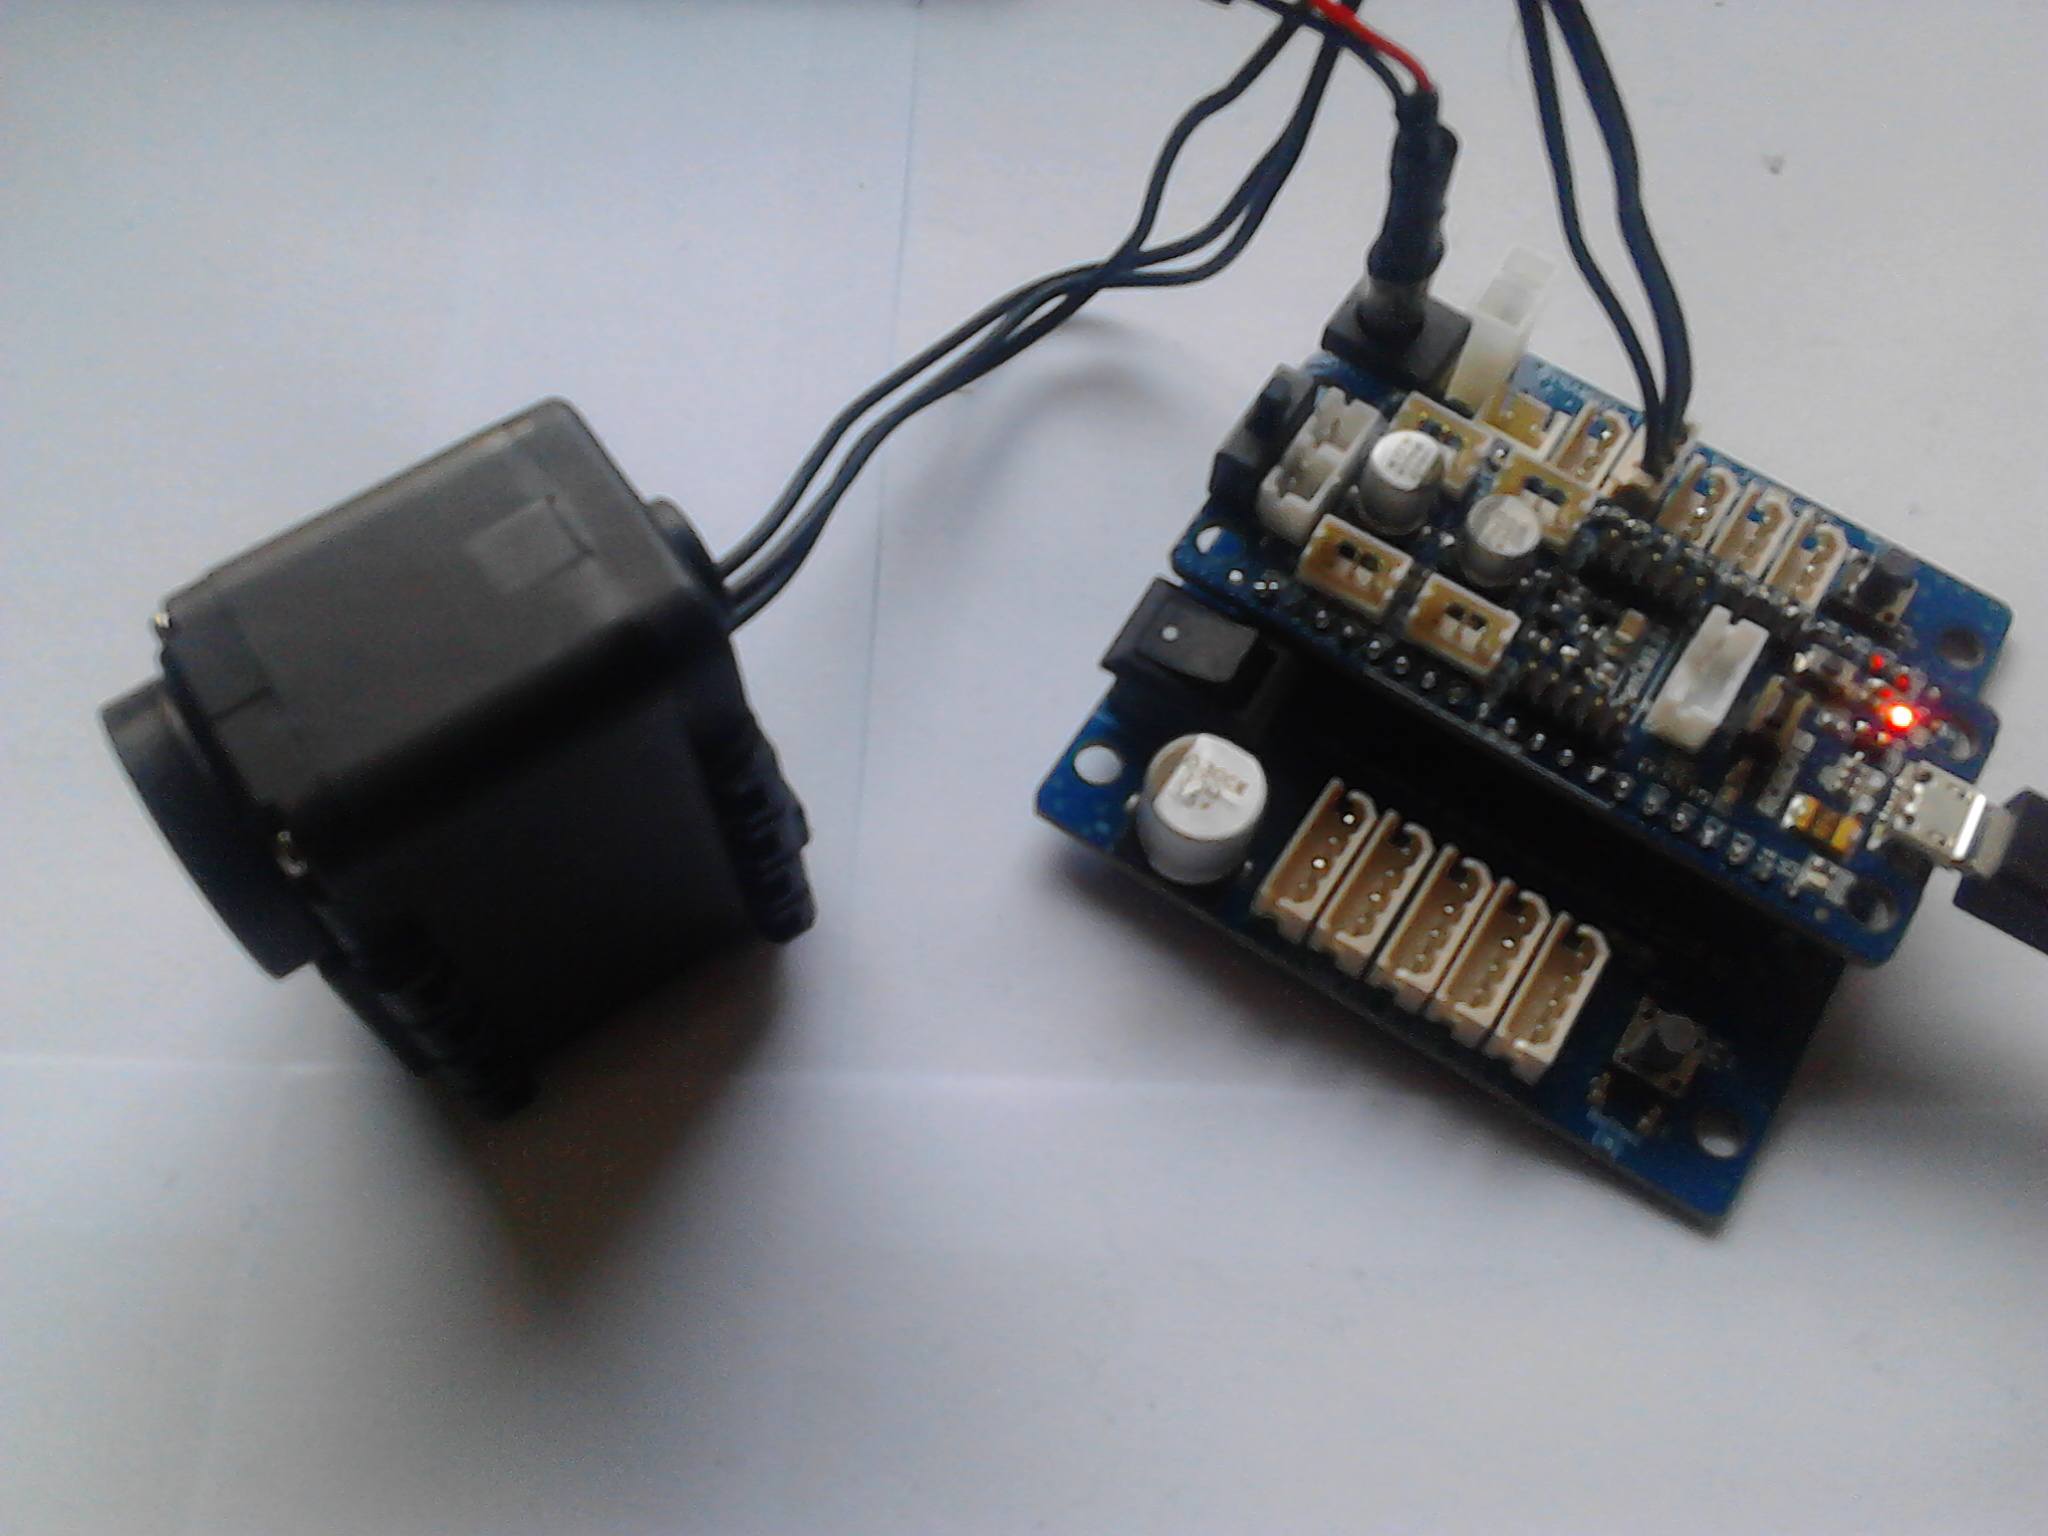
\includegraphics[width=0.85\textwidth]{03_Grafiken/Grundlagen/Testaufbau/Komponenten.jpg}
	\caption[Testaufbau]{Testaufbau}
	\label{fig:Testaufbau}
\end{figure}



\subsection{Programmierung}
\subsubsection{OpenCM Code}
Das OpenCM Board wird mit der gls{ide} Robotis OpenCM (modifizierte 
Arduino-Umgebung) programmiert, da das Programm sehr schlicht gehalten wird.
Der Speicherplatz von OpenCM ist stark begrenzt, sodass dieses nur als 
Befehlsverteiler fungiert.\\
Das bedeutet, dass ein übergeorndneter Rechner (geplant ist Raspberry Pi) eine 
in C\# geschriebene \gls{hmi} enthält mit der die komplette Regelung aktiviert 
und (in gewissen Mae) modifiziert werden kann.\\
Das Board OpenCM empfängt die vom Rasbperry Pi gesendeten Befehle und leitet 
diese an die entsprechenden Aktoren weiter.

Das Programm, welches auf dem OpenCM-Controller läuft ist in 
\ref{lst:OpenCMcode} dargestellt.\\
In Zeile 1-3 erfolgt das Definieren des seriellen Bus, welche verwendet werden 
können. Da das Extension Board zusammen mit dem OpenCM Controller Verwendung 
findet wird in Zeile 9 der Bus 3 übergeben.\\
Jeder Aktor erhält eine ID (zwischen 0 und 253) und ist aktuell (wie in Zeile 4 
zu sehen) auf 1 gesetzt. 
Die Befehle, welche an den Servomoter geschickt werden können, um Daten zu 
setzen oder abzurufen sind in \ref{tab:CommandsDynamixel} dargestellt. In Zeile 
6 erfolgt die Definition des Befehls 30, die den Aktor zu einer Position (0-300 
$[$deg$]$, bzw. 0-1024).\\
In der setup-Routine (Zeile 11-15) erfolgt das Setzen der Baudrate (s. 
\ref{tab:baudrate}) und des Bewegugnsmodus (Joint oder Wheel) für den 
entsprechenden Aktor. 
Sobald Daten auf der seriellen Schnittstelle vorliegen werden diese in Zeile 
19-23 mit der Funktion getValue() abgerufen und an die Funktion Dxl.writeWord() 
(s. \ref{lst:dxlWriteWord} übergeben.
\label{lst:dxlWriteWord}
\begin{lstlisting}[language=java, caption=Funktion dxlWriteWord]
void dxl_write_word(
   int id,
   int address,
   int value
);
\end{lstlisting}

Die Funktion getValue() liest die Anzahl der gesendeten Zeichen und splittet 
diese auf in die ID, den Befehl und den Wert für den Befehl (Zeile 17-XX).

\label{lst:OpenCMcode}
\begin{lstlisting}[language=java, caption=OpenCM-Programm]
#define DXL_BUS_SERIAL3 3
#define ID_NUM 1
#define DIM_ID_ARRAY 3
#define DIM_CMD_ARRAY 2
#define DIM_VAL_ARRAY 4

Dynamixel Dxl(DXL_BUS_SERIAL3);
  int id;
  int command;
  int sollPosition;

void setup() {
  Dxl.begin(3);
  Dxl.jointMode(ID_NUM);
}

void loop() {
   id = getValue();
   command = getValue();
   sollPosition = getValue();
   if((id != -1) & (command != -1) & (sollPosition != -1)) Dxl.writeWord(id, 
   command, sollPosition);
   delay(100);
}

int getValue(){
  int inValue;
  int cntr;
  int motorId[DIM_ID_ARRAY];
  int command[DIM_CMD_ARRAY];
  int value[DIM_VAL_ARRAY];
   
  // Check if there is something to receive
  cntr = SerialUSB.available();  
  if(cntr>0){
    // Read the first parameter to the first semicolon
  for(unsigned int i=0; i < cntr;i++){
      inValue = (SerialUSB.read())-48;
      if(inValue != 11) {
        motorId[i] = inValue; 
      }
      else return calcValue(motorId, i,calcMult(i));;
    }
    }
    else return -1;
  } 

// Caclulate the multiplicator
int calcMult(int steps){
    int multiplicator = 1;
    
    for(unsigned int i=0; i < steps-1;i++){
      multiplicator = multiplicator*10;
   }
   return multiplicator;
}

// Calculate the value
int calcValue(int data[], int dim, int factor){
  int retVal = 0;

    for(unsigned int i=0; i <= dim-1;i++){
      retVal = retVal+(data[i]*factor);
      factor = factor/10;
   }  
   return retVal;
}
\end{lstlisting}

\subsubsection{Matlab Code}
Die entsprechenden Befehle können über ein Matlab-Skript (s. 
\ref{lst:matlabScript}) an das Board OpenCM gesendet werden. 

\label{lst:matlabScript}
\begin{lstlisting}[language=java, caption=Matlab-Skript]
function ComDeltaRobot()    
    pTime = 0.8;
    
    PortID = serial( 'COM3' );
    set( PortID,'BaudRate',9600, 'StopBits', 2);
    
    fopen( PortID );
    
    fprintf(PortID,'1;30;55;');
    pause(pTime);
    
    fprintf(PortID,'1;30;0;');
    pause(pTime);

    fprintf(PortID,'1;30;55;');
    pause(pTime);
    
    fprintf(PortID,'1;30;0;');
    pause(pTime);
    
    OutPort = instrfind('Port','COM3');
    NewObjs = instrfind;
    fclose(NewObjs);   
end
\end{lstlisting}

\section{Nachrichtenaufbau}
\label{sec:Nachrichtenaufbau}
Jede Nachricht, die von dem Master-Computer (Raspberry Pi) gesendet und von dem 
OpenCM-Board korrekt empfangen werden soll, muss folgendes Format aufweisen:

Nachricht = \{ID\};\{COMMAND\};\{VALUE\};

Die Werte für \{ID\} sind für den entsprechenden Servomotor bestimmt und ist 
auf den Wertebereich zwischen 0 - 253 beschränkt.\\
Die Werte für \{COMMAND\} sind der Tabelle zu entnehmen, die auf folgender 
Website \url{} zu finden ist. Die wichtigsten Befehle sind zur Übrsicht in 
\ref{fig:commands} dargestellt.

\begin{figure}[H]
	\centering
	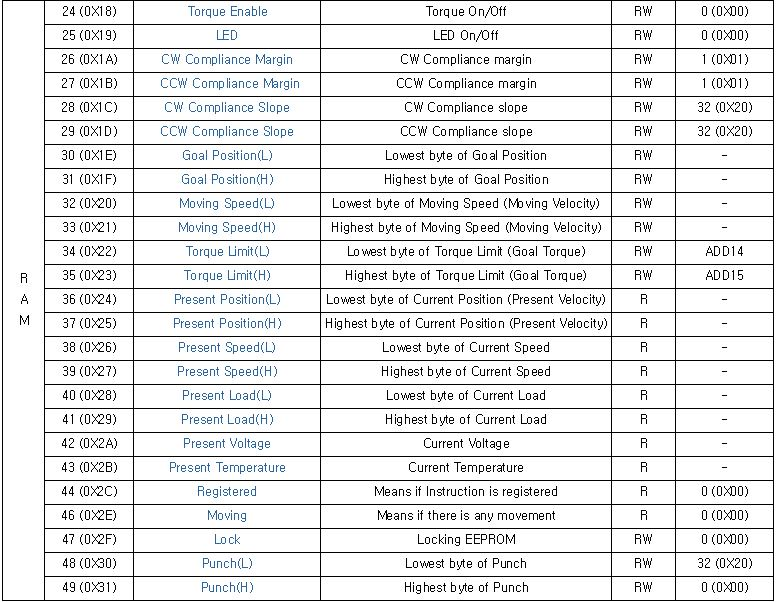
\includegraphics[width=0.85\textwidth]{03_Grafiken/Grundlagen/Nachrichtenaufbau/CommandsTable.jpg}
	\caption[Wichtige Kommandos]{Wichtige Kommandos}
	\label{fig:commands}
\end{figure}

Der Wert \{VALUE\} ist zunächst dafür vorgesehen, um den Drehwinkel für den 
Aktor angeben zu können. Um einen Servomotor mit der ID = 1 auf 55 $[$deg$]$ zu 
positionieren muss folgender String übertragen werden: \textbf{1;30;55;}

Auf dem übergeorndeten Rechner kann dann eine Regelstruktur implementiert 
werden, die entsprechende Kommandos an die jeweils beteiligten Aktoren sendet.






	\chapter{Ausblick}

	
	\pagenumbering{Roman}	% R�mische Seitenzahlen (IV)
	\bibliography{02_Inhalt/Literatur}
	\appendix 
%\refstepcounter{chapter}
%
% Anhang
%
%\section{SectionAnhang} 
% %\subsection{SubsectionAnhang}
%% ------------------------------
% Bild im Anhang
% ------------------------------
\begin{figure}[H]
	\centering
		
\includegraphics[width=0.85\textwidth]{03_Grafiken/PseudoImage.jpg}
	\caption[Bild im Anhang]{Bild im Anhang}
	\label{fig:BildAnhang}
\end{figure}
%\newpage
%\subsection{SubsectionAnhang}
%\label{app:SubsectionAnhang}
%\input{99_Anhang/...}
%
% Weiteres im Anhang
%
%\newpage
%\section{Listings}
%\label{app:Quellcode}
%\subsection{Beispiel-Anwendung HelloWorld}
%\label{abbCode:moduleServerComm}
\begin{lstlisting}[language=java, caption=Task ServerComm - Modul ServerComm]
PROC main()
    WHILE TRUE DO
        waitForClients;
    ENDWHILE
ENDPROC    
(...)
PROC waitForClients()
     TEST state
     CASE 1:
			(...)
     CASE 4:			
         WHILE listening DO
             IF i<=MAX_CLIENTS THEN					
                 SocketAccept server_socket,client_socket{i}\Time:=WAIT_MAX;    
					(...)
					ENDIF
         ENDWHILE
 				FOR i FROM 1 TO 25 DO
 					IF (bufferStateEvent{i}) THEN
 						SocketSend client_socket{1}\Str:=sendbufferEvent{i};
 						sendbufferEvent{i} := "";
 						bufferStateEvent{i} := false;
 						WaitTime 0.08;
 					ENDIF					
					(...)										
 				ENDFOR
     DEFAULT:
     ENDTEST   
ENDPROC    

    ERROR
        IF ERRNO=ERR_SOCK_CLOSED THEN
		(...)
        IF ERRNO=ERR_SOCK_ADDR_INUSE THEN
		(...)
        IF ERRNO=ERR_SOCK_TIMEOUT THEN
		(...)
    ENDPROC

    PROC initSocket()
        SocketClose server_socket;
        SocketClose client_socket{1};
		(...)
        listening:=TRUE;
		clientConnected:=FALSE; 
    ENDPROC
\end{lstlisting}

%\input{99_Anhang/...}
%\newpage
%\section{SectionAnhang}
%\label{app:SectionAnhang}
%\subsection{SubsectionAnhang}
%\input{99_Anhang/...}

%
% Erklaerung
%
\lstlistoflistings
\listoffigures
\listoftables
%\printglossary[type=\acronymtype]%, style=listdotted
%\printglossary			
    
	
%%%%%%%%%%%%%%%%%%%%%%%%%%%%%%%%%%%%%%%%%%%%%%%%%%%%%%
\end{document} 
% ----------------------------------------------
